\chapterimage{Figures1_3/Introimage.png} % Chapter heading image
%Einstein Telescope artits impression copyright Nikhef
%\section{Introduction}
\chapter{Introduction}
\label{sec:Intro}
\pagenumbering{arabic}
\setcounter{page}{1}
%\vspace{-1.5cm}
In this chapter we review subsystem requirements for \ac{3G} detectors,  state of maturity and major \ac{RaD} needs faced to construct massive new facilities, far larger than current facilities,  and operate in them detectors with \ac{3G} sensitivity.
An overview of required rough timelines to reach installation maturity is depicted in figure~\ref{fig:maturity}. 

\begin{figure}[h]
\centering
\includegraphics*[width= \textwidth]{Figures/3G_Readiness_Levelsblue.pdf}
\caption{Approximate timelines for the required maturity levels for \ac{3G} instruments and resource levels needed from now to installation of the first phase. The estimates for the required \ac{RaD} resource level shown on the right hand side only include investment (not \ac{RaD} person costs, assumed to be supplied form the labs) and are roughly categorized into \textit{low, mid} and \textit{high}.\\
}
\label{fig:maturity}
\end{figure}

The figure shows required maturity levels for the various subsystems, depending on the foreseen time of installation and anticipated lead times. Infrastructure and facilities have the longest development lead times and thus will have to reach maturity earliest, followed by the other subsystems in the sequence of installation. The timings for the lower maturity level (ML) ML1 - ML3 (relative to the highest level ML4) depend on the duration required between the individual steps; e.g. once technical readiness is achieved for core optics it still takes a few years to demonstrate full scale prototypes and manufacture the final optics substrates through a pathfinder process. Despite considerable differences in designs for the proposed \ac{3G} observatories (\acs{ET} and \acs{CE}), large variations within the subsystems and an inevitable uncertainty in timelines, we nonetheless attempt to summarize the timelines for each subsystem in a single bar in figure~\ref{fig:maturity}. The resources required to reach operational readiness are roughly divided into low, mid and high, with indicative financial investments for \ac{RaD} for the various subsystems over the entire period from now to the start of installation. 
The highest costs for the detector elements (as distinct from the civil and vacuum construction) are expected for developing the capabilities to manufacture the main optics (presumably fused silica and silicon) and for the development of coatings and coating facilities. Producing ultra-pure optics substrates of approx. 200-300\,kg weight requires an international effort and tight collaboration with industry. Developing coatings of outstanding optical quality and uniformity over the whole mirror surface, combined with the required low mechanical losses at room temperature and cryogenic temperatures is currently regarded as the biggest hurdle to overcome for building \ac{3G} gravitational wave observatories. International collaboration and building redundancy in coating capabilities is essential for success. 
In particular for underground infrastructures and facilities, \ac{RaD} will incur significant costs for exploration and prototyping. Exploratory efforts have already been started at the \ac{ET} candidate sites. In the construction phase, building the infrastructure and facilities will be the biggest cost items and consequently have the largest cost saving potential. \ac{RaD} efforts to minimise costs while satisfying the strict technical demands is mandatory. 
Achieving timely progress in the development of enabling technologies for \ac{3G} detectors will require global collaboration and coordination. A broad, global coherent detector \ac{RaD} program is needed now addressing key technological challenges in the next 5-7~years. In order to facilitate timely development, we propose four broad recommendations on top of the earlier presented subsystem specific recommendations. 
\begin{itemize}
\item \textbf{Recommendation 1}:  An international \ac{3G} \ac{RaD} coordination committee should be formed, with broad and inclusive membership representing \ac{GW} groups across the world.

 A series of workshops on enabling technologies shall be held in order to stimulate exchange of ideas and allowing (if deemed useful) for coordination of the person-power intensive experimental activities.  Each of the major \ac{RaD} tasks should generate a list of  goals with quantitative metrics,  timelines and required resources.   Activities requiring global collaboration and coordination should be laid down and pathways identified.

\item \textbf{Recommendation 2}:  International consortia should be formed to work on key \ac{RaD} challenges and opportunities with industrial partners, establish a governance and organisational structure with authority and seek funding through joint proposals submitted across funding agencies.

\item \textbf{Recommendation 3}: 
National funding agencies should maintain a proactive role in ensuring that the \ac{RaD} activities are well-focused and effective.  Coordination of funding plans through\ac{GWAC} would be a first step, followed by supporting the role of the international \ac{3G} \ac{RaD} coordination committee (recommendation 1) in organizing the global effort.  This is likely to require increased funding for staff and instrumentation to enable the required long-term research programs at relevant laboratories and prototype interferometers.

\item \textbf{Recommendation 4}: Existing \ac{GW} collaborations embrace \ac{3G} \ac{RaD} tasks and integrate them into their programs and deliverables, in order to ensure sufficient support for the long-term future of the field (as it has been done so successfully for \ac{2G} \ac{RaD} during the operation of the initial detectors). Over the next 5 years, mature \ac{2G} enabling technologies (e.g. 1064\,nm laser, fused silica optics, coatings) will need to be scaled up and shown ready for application in \ac{3G} facilities.
\end{itemize}


The new \ac{3G} facilities will be designed to accommodate successive generations of detectors with increasing sensitivity as the technology evolves and new ideas emerge as has happened with existing facilities. The infrastructures which initially housed the "first generation detectors" (\acs{1G}) (\textit{\acs{LIGO}}~\cite{Abbott2009} and \textit{\acs{Virgo}}~\cite{VirgoStatus2008}), now house the second generation: the \textit{\acs{aLIGO}}~\cite{AdvancedLIGO2015} detectors, \acs{AdVirgo}~\cite{AdvancedVirgo2015}, along with \acs{LIGOIndia} and \acs{KAGRA}. \\
Currently (circa 2021)  Advanced LIGO and Advanced Virgo have completed  their third observing run. There are plans for further upgrading these 2G detectors towards \acs{a+LIGO}, \acs{AdVirgo+}~\cite{Zucker:LIGOAplus, Cagnoli:VirgoAplus}.  Furthermore, completely new detectors, such as  \acs{Voyager} \cite{VoyagerDCC2018} and the Neutron star Extreme Matter Observatory \acs{NEMO}~\cite{NEMO2020}, referred to as  \acs{2.5G}  detectors, may later be installed in the existing facilities or new facilities of a similar scale.

Therefore, in the mid 2030s we envision a network of new detectors, \ac{CE} and \ac{ET}, in new, longer-baseline \ac{3G} facilities, along with detectors that use \ac{3G} technology within \ac{2G} facilities, such as \ac{Voyager} and \ac{NEMO}, in addition to the potentially still operational, upgraded \ac{2G} detectors.
The first instruments to be installed in the new \ac{3G} Observatories will be 10 to 20 times more sensitive than the current \ac{2G} instruments above 100\,Hz (Fig.~\ref{fig:3GSens}). The improvement factor exceeds 100 around 10\,Hz and thousands below 10\,Hz. The key parameters of \ac{2G} and \ac{3G} instruments are summarized in Table~\ref{Tab:FutIfos}. The \ac{3G} facilities are being designed with lifetimes up to 50 years in order to house detectors far more sensitivity that the initially  proposed ET and CE  designs.  Strategies for \ac{3G} will be modified according to observations made with current detectors, evolution in the science case, technology readiness and funds available. Nonetheless, this \acs{GWIC} \ac{3G} report represents a milestone community vision for the future of ground based gravitational wave observations. 

 Section~\ref{sec:Fac_Inf} will cover the \ac{RaD} needed to select suitable sites and build such large, long-lifetime facilities in a cost efficient way. The remainder of this chapter will focus on the \ac{RaD} required to deliver the first detectors operational in these \ac{3G} facilities.  Currently, there are two main concepts for these detectors, \acf{ET}~\cite{ET2011}, a 10-km triangular underground detector, and \acf{CE}~\cite{CosmicExplorer2017}, a 40-km above-ground L-shaped detector. These concepts, along with the \ac{2.5G}  detector \ac{Voyager}~\cite{Voyager:Inst,VoyagerDCC2018} are highlighted in Box~\ref{Box:GWOs}.

Planning for the \ac{3G} detectors began more than 20 years before they are envisioned to become operative. This was based on experience with past and current detectors, for which there was a lead time of 15 years or more from conception to operation. Assuming a 2035 start date for initial \ac{3G} operations, preceded by five years of construction and five years of commissioning, it is likely that only technologies with mature \ac{RaD} in 2025 will feed into final design and engineering for the initial \ac{3G} detectors. 

Despite their differences in design, the \ac{3G} detectors \ac{ET} and \ac{CE} rely on similar 'enabling technologies' -- the main pillars on which the predictions of sensitivity are based. These technologies are used to mitigate 'fundamental noise sources' affecting the instruments, in particular: \textbf{Quantum noise} associated with the laser light fields is modified by high laser power, quantum squeezing, massive mirrors and interferometer topology; \textbf{Thermal noise} in mirror substrates, coatings and suspensions is modified by temperature and material properties (and their behaviour as a function of temperature); and \textbf{Newtonian noise} caused by the gravitational forces of moving masses (such as air, the ground, and machinery) is modified by the location of the sites and subtraction schemes.  Similarly supporting technologies such as control techniques and methods to  mitigate  a forest of noise technical  are issues common to all interferometer designs.\\
These considerations are interdependent and have implications for the detector designs. For example, using low temperatures to reduce Brownian noise requires a departure from the fused silica optics used in Advanced LIGO and Advanced Virgo. Sapphire and Silicon are promising low temperature materials. Silicon would require changing the operating wavelength to 1.5 -- 2\,\micro m, necessitating the development of a new suite of light sources, optical components and detectors. Considering the material properties as a function of temperature and wavelength as well as the ability to handle high optical power while minimizing noise during heat extraction from the core optics leads to four possible operating temperatures: room temperature and the cryogenic temperatures of 123\,K, 20\,K and below 5\,K.  At this time we are not able to make these decisions. The final technology choices for the first interferometers in the \ac{3G} facilities will depend on \ac{RaD} progress across the various subsystems.  It  will require intensive sensitivity trade studies informed by science goals and is beyond the scope of this report.  Indeed different collaborations  may choose different optimizations.   In a conservative scenario, the first instruments could use technologies already proven in  \ac{2G} facilities.  This is the option currently favoured by the Cosmic Explorer collaboration, referred to as \acs{CE1}.




%Two detector epochs are envisioned 
% post advanced detector baseline sensitivities 
%to follow the advanced detectors over the next 25\,years: upgrades in existing facilities; % operating at 1\,$\mu m$ wavelength; 
%and new detectors in new, longer baseline, third generation (3G) facilities. 

%The \ac{3G} facility infrastructure can to some extent be decoupled from the initial \ac{3G} instruments. 

% There are currently two conceptual designs for such \ac{3G} facilities:  The Einstein Telescope (ET) and Cosmic Explorer (CE). A short description is given in Box \ref{Box:GWOs} and the key parameters of \ac{2G} and \ac{3G} instruments are summarized in table \ref{Tab:FutIfos}.
%The Einstein Telescope (ET) is envisaged as an underground facility capable of housing three pairs of detectors in a nested triangular vacuum envelope with three 10\,km sides. Cosmic Explorer is proposed to be a single L-shaped facility with two 40\,km arms. The most effective \ac{3G} network would incorporate a pair of widely separated Cosmic Explorers working in unison with the Einstein Telescope~\cite{Hall:2019xmm}.


 % quantum noise, thermal (Brownian) noise and Newtonian noise. 
%Seismic noise and residual gas noise had been listed as fundamental noises, but as they are treatable by more expensive technology we do not list them as fundamental here.

\begin{wrapfigure}{r}{0.65\textwidth}
%\begin{figure}[ht]
\centering
\includegraphics*[width= 0.64\textwidth]{Figures/noises_percentiles-Voyager.pdf}
\caption{Target sensitivity curves for \ac{3G} gravitational-wave detectors \acf{ET}~\cite{ET2011}, shown in green, and \acf{CE}~\cite{CosmicExplorer2017}, shown in pink, compared with the design sensitivity of Advanced LIGO, shown in blue. 
%and the goal sensitivity for Voyager (orange curve). 
The shades of the curves represent sensitivity to sources with differently distributed locations.}
\label{fig:3GSens}
%\end{figure}
\end{wrapfigure}



% Prototyping such technology may include testing performance and science capability in an existing \ac{2G} facility. The term "Voyager" is used to describe a detector in a \ac{2G} facility that would prototype \ac{CE} phase 2 technology whilst significantly improving detection range. 

In this chapter, we assess the state of \ac{RaD} for \ac{3G} enabling and supporting technologies  toward readiness before the end of the decade while also looking ahead to the \ac{RaD} that will continue as a necessary preparation for subsequent \ac{3G} upgrades. Each section contains an outlook for the activity and recommendations on how to best  progress the \ac{RaD} globally.  We begin by presenting a brief overview on the basics of gravitational wave detection, and introduce the main subsystems that make up an interferometer. Then in section \ref{sec:Fac_Inf} we address requirements and design aspects of the \ac{3G} infrastructure. In Sections \ref{sec:Core_optics} to \ref{sec:Newtonian_Noise} we consider the state of the art in enabling technologies, the \ac{RaD} needed in each area, the level of resources needed (broadly bracketed as high, medium, low), and how the \ac{RaD} should be focused in order to deliver fully tested subsystems for timely installation in new \ac{3G} facilities.  The analysis suggests prototyping \ac{3G} technology including new test facilities and use of existing long baseline facilities. 



Sections~\ref{sec:Core_optics} and \ref{sec:Coatings} describe the closely related subjects of core optics and coatings, while Section~\ref{sec:Cryogenics} describes cryogenics, and Section~\ref{sec:Suspensions_Isolation} covers suspensions and seismic isolation systems.
A common theme among these chapters is thermal noise, described in Box~\ref{Box:Thermal}, which is the primary consideration for many choices in optics, coatings, suspensions, and operating temperature. 
Chapter~\ref{sec:Newtonian_Noise} describes Newtonian noise and its connection with facility choices and reliance on modeling and subtraction schemes. 
In addition to the fundamental noises described above, a myriad of technical noise sources and control issues can limit interferometer performance: parametric instabilities, scattered light, and noise originating from auxiliary optics and control systems. 
The current state of the art in these areas, \ac{RaD} needed, and coordination for \ac{3G} are reviewed in sections \ref{sec:Aux-optics} and \ref{sec:Sim_Controls}. 
Finally, Section~\ref{sec:Calibration} describes plans for accurately calibrating the instruments to levels that will enable the dramatic science described in the first part of this report.   We end in the summary  by proposing  four broad recommendations designed to optimise global \ac{RaD}  resources in order to make timely progress.

\newpage
%%%%%%%%%%%%%%%%%%%%%%%%%
%% BEGIN DETECTORS BOX
%%%%%%%%%%%%%%%%%%%%%%%%%

\begin{DetBox}{\bf Future Gravitational Wave Observatories}
\stepcounter{boxcount}
%see definition in structure.tex
\label{Box:GWOs}
\begin{tcolorbox}[standard jigsaw,colback=amber!10!white,colframe=red!70!black,coltext=black,size=small,  title=The Einstein gravitational--wave Telescope (ET)] 
%\begin{tcolorbox}[standard jigsaw,colback=amber!10!white,colframe=red!70!black,coltext=black, size=small, title=The Einstein gravitational--wave Telescope (ET)] 
\begin{wrapfigure}{r}{0.4\linewidth}
\vspace{-10pt}
\includegraphics*[width=0.4\textwidth]{Figures/ET_Thumb.png}
\label{fig:ET_Thumb}
\vspace{-25pt}
\end{wrapfigure}
ET~\cite{ET2011} is 
%the European concept 
 a concept for a third generation gravitational-wave \emph{observatory}
 likely with a location in Europe. 
 To reduce the effects of seismic motion, the \ac{ET} concept calls for the site to be located at a depth of about 100\,m to 200\,m below ground. In its final configuration it shall be arranged as an equilateral triangle of three interlaced detectors, each consisting of two interferometers. The configuration of each detector dedicates one interferometer \ac{ET-LF}  to detecting the \textbf{L}ow \textbf{F}requency components of the gravitational-wave signal (2--40\,Hz), while the other one \ac{ET-HF}   is dedicated to the \textbf{H}igh \textbf{F}requency components, called a "xylophone" design. Each interferometer will have a dual-recycled Michelson layout with about 10\,km long \ac{FP}. In \ac{ET-LF} , which operates at cryogenic temperature, thermal, seismic, gravity gradient and radiation pressure noise sources are particularly suppressed; in \ac{ET-HF} , sensitivity at high frequencies is improved by high laser light power circulating in the \ac{FP}  cavities and the use of frequency-dependent squeezed light technologies.
\end{tcolorbox}


\begin{tcolorbox}[standard jigsaw,colframe=antiquefuchsia!80!black,colback=antiquefuchsia!20!white,opacityback=0.6,coltext=black,size=small, title=Cosmic Explorer (CE)] 
\begin{wrapfigure}{r}{0.4\linewidth}
\vspace{-10pt}
\includegraphics*[width=0.4\textwidth]{Figures/CE_Thumb.jpg}
\label{fig:CE_Thumb}
\vspace{-20pt}
\end{wrapfigure}
CE~\cite{CosmicExplorer2017} is a concept for an L-shaped above-ground observatory with 40\,km arm-length, operating a dual recycled Michelson interferometer with \ac{FP}  arm cavities, with possible site location in the US or/and in Australia. 
% CE~\cite{CosmicExplorer2017} is a US concept that envisions 40\,km long arms and new technologies to achieve a factor of 10 or more strain sensitivity improvement over the current generation of gravitational-wave detectors. 
% As with LIGO, it will employ a dual recycled Michelson interferometer with \ac{FP}  arm cavities and be implemented in stages. 
Its initial phase, called \ac{CE1}, will employ scaled-up \emph{Advanced LIGO technology} including 440\,kg fused silica test masses, 1.5\,MW of optical power, and frequency-dependent squeezing. 
% Frequency-dependent squeezing will improve the quantum limited sensitivity by a factor of three. 
A major upgrade, \ac{CE2}, will properly exploit the new facility by either using \emph{Voyager technology} such as silicon test masses and amorphous silicon coatings operating at 123\,K, with $1.5$ or $2\,\mu m$ laser light and 3\,MW of optical power in its arm cavities or continue to use room temperature A+ technology pushed to its limits.

\end{tcolorbox}

%\begin{tcolorbox}[standard jigsaw,colframe=azure!70!black,colback=azure!20!white,opacityback=0.6,coltext=black, size=small, title= Voyager,sidebyside,righthand width=.3\textwidth,sidebyside gap=6mm,lower separated=false]
\begin{tcolorbox}[standard jigsaw,colframe=azure!70!black,colback=azure!20!white,opacityback=0.6,coltext=black, size=small, title=Voyager]

\begin{wrapfigure}{r}{0.4\linewidth}
\vspace{-10pt}
\includegraphics*[width=0.4\textwidth]{Figures/Voyager_Thumb.png}
\label{fig:Voyager_Thumb}
\vspace{-20pt}
\end{wrapfigure}

Voyager~\cite{Voyager:Inst,VoyagerDCC2018, VoyagerDCC2019} is the tentative concept for a new detector in the current facilities, designed to maximize the observational reach of the infrastructure and demonstrate the key technologies to be used for \ac{3G} observatories in new infrastructures.
Voyager proposes to use heavy (ca.\,200\,kg) cryogenic mirrors with improved coatings and upgraded suspensions made of ultra-pure silicon at a temperature of 123\,K in the existing vacuum envelope and a laser wavelength of $\sim1.5\,-\,2\,\mu m$. 
A further factor of 3 increase in BNS range (to 1100\,Mpc) is envisioned along with a reduction of the low frequency cutoff. %down to 10 Hz.
 In the context of this report we use the term \emph{Voyager Technology} for this type of technology irrespective of plans to implement it in any of the existing or future infrastructures.  Recently a detector, called \ac{NEMO} \cite{NEMO2020}, has been proposed. It  may use aspect of  Voyager technology but is optimised for the kHz band in order to measure the neutron star state equation of state. 
\end{tcolorbox}

\end{DetBox}


%%%%%%%%%%%%%%%%%%%%%%%%%
%% END DETECTORS BOX
%%%%%%%%%%%%%%%%%%%%%%%%%
\newpage

\begin{table}[ht]
\centering
\begin{tabular}{|l|l|l|p{1.6cm}|l|l|l|l|}
\hline
 % \multicolumn{8}{|c|}{Current and Future Interferometers}\\ 
 %\hline
 &aLIGO / AdV &A+/V+ &KAGRA &CE 1 &CE 2 &ET-LF &ET-HF\\
\hline
Arm Length [km] & 4 / 3 &4 / 3& 3& 40& 40& 3x10$^*$ & 3x10$^*$\\
\hline
Mirror Mass [kg]& 40 / 42& 40& 23& 440& 470& 211& 200\\
\hline
Mirror Material& silica& silica& sapphire& silica& silicon& silicon& silica\\
\hline
Mirror Temp [K]& 295& 295& 20& 295& 123& 10& 290\\
\hline
Suspension Fiber& 0.6m/0.7m& 0.6m& 0.35m& 2m& 2m& 2m& 0.6m\\
& SiO2& SiO2&Al2O3&SiO2&Si&Si&SiO2\\
\hline
Fiber Type& Fiber& Fiber& Fiber& Fiber& Ribbon& Fiber& Fiber\\
\hline
Input Power [W]& 125& 125& 70& 140& 280& 3& 500\\
\hline
Arm Power [kW]& 710 / 700& 750& 350& 1500& 3000& 18& 3000\\
\hline
Wavelength [nm]& 1064& 1064& 1064& 1064& 2000& 1550& 1064\\
\hline
\acs{NN} Suppression& 1& 1& 1& 2& 10& 1& 1\\
\hline
Beam Size [cm]& (5.5/6.2) / 6& 5.5/6.2& 3.5/3.5& 10/13& 14/18& 9/9& 12/12\\
\hline
\acs{SQZ} Factor [dB]& 0& 6& foreseen& 6& 10& 10& 10\\
\hline
Filter Cavity & none& 300& unknown& 4000& 4000& 10000& 500\\
Length [m] &&&&&&&\\
\hline
\end{tabular}
\caption{Key parameters of the current Advanced detectors, their enhancements, LIGO A+ and AdVirgo +, the two phases of Cosmic Explorer, \ac{CE1} and \ac{CE2}, and the two interferometer types of Einstein Telescope. $^*$\ac{ET} will have an angle of 60$\deg$ between the detector arms}
\label{Tab:FutIfos}
\end{table}

\begin{Infobox}{\bf Thermal Noise in Gravitational Wave Detectors}
\stepcounter{boxcount}
%\label{Box:Thermal}
%\paragraph{Infobox Thermal Noise in gravitational wave detectors}
Thermal noise is one of the fundamental noise sources limiting \ac{2G} detectors over a considerable frequency range. The main contributions come from Brownian noise of the mirror suspensions, substrates and coatings and thermo-optic (thermo-elastic plus thermo-refractive) noise of substrates and coatings. The relation between the dissipation and the power spectrum (single sided) of the noise is described by Callen's Fluctuation-Dissipation Theorem~\cite{CaWe1951, Kubo:FDT, Callen:1959} and is given by:
\begin{equation}
S_x(\omega) = \frac{4\,k_B T}{\omega^2} \left| \mathrm{Re} \big[ Y(\omega) \big]\right| .
\end{equation}
\label{eq:FDT}
with \acf{k_b}, \acf{omega} , \acf{T} and \acf{Y}, defined as
\begin{equation}
Y(\omega) = i \omega\frac{X(\omega)}{F(\omega)} \, ,
\end{equation}
where \acs{DNA} and \acs{FNA} are the Fourier components of the displacement of the system and force applied leading to the displacement, respectively. The real part of the admittance is proportional to mechanical losses, hence low noise requires low mechanical losses.
Operating the mirrors and suspensions at reduced temperature reduces thermal noise since the 
%$x(\omega)$ 
\ac{DNA} scales with $\sqrt{T}$. 
%More significantly, many material properties of mirror substrates (e.g., for sapphire and silicon) and coatings (e.g., AlGaAs, AlGaP, $\alpha$-Si) scale favorably with decreasing temperature. 
%This makes the improvement in the noise potentially better than $\sqrt{T}$. Most glasses, e.g. fused silica, have increased mechanical losses at cryogenic temperatures, making them unsuited for use at cryogenic temperatures. 
More significantly, many material properties of mirror substrates and coatings depend on temperature, and hence influence the temperature dependence of thermal noise.
Fused silica, like most other glasses, has increased mechanical losses at cryogenic temperatures, making it unsuitable as substrates at cryogenic temperatures, making crystalline materials (Sapphire, Silicon) the prime candidates for low temperature operation.
Most amorphous oxide coatings show higher mechanical losses at cryogenic temperatures while the losses of crystalline or semiconductor coatings improve. The latter ones suffer from other drawbacks, e.g. optical absorption, though.
Further dependence of coating thermal noise on coating parameters is shown in Appendix~\ref{sec:Appendix_Coatings}, Figure~\ref{fig:Thermal_Noise}.
\label{Box:Thermal}
\end{Infobox}
%\end{tcolorbox}

%\begin{tcolorbox}[standard jigsaw,colframe=ocre,colback=blanchedalmond!10!white,opacityback=0.6,coltext=black,oversize,  size=small, title=Infobox~\theboxcount: Gravitational Wave Detection] 


\section{Gravitational Wave Detection Basics}
Gravitational waves induce tiny changes in separation between widely spaced 'test masses'. The instrumental challenge is to measure these tiny changes. Audio band detectors use laser interferometry, where the interferometer mirrors are the test masses at the ends of long baselines whose length changes are measured. The basis of all present and next generation gravitational wave detectors is a dual recycled Fabry-Perot arm cavity Michelson interferometer as sketched in figure\,\ref{fig:ifo_layout}. 
%\begin{wrapfigure}{l}{1.1\columnwidth}
\begin{figure}[ht]
\includegraphics*[width=\textwidth]{Figures/InterferometerSchematicSubsystemColourSAS.pdf}
\caption{Schematic representation of an interferometric gravitational wave detector. Subsystems as used in this report are indicated by the colored backgrounds. The borders between subsystems are not sharply defined and somewhat arbitrary.}
\label{fig:ifo_layout}
\end{figure}
%\end{wrapfigure}

Being quadrupolar radiation, a passing \ac{GW}  alternately expands and then contracts one arm (e.g. $L_x$) of the interferometer whilst it contracts and then expands the arm perpendicular to it ($L_y$).  The effect is extremely small: expressed as a relative length change, $\delta L/L$, it is less than $10^{-22}$! The arm cavities increase the phase change imposed on the light. Interfering the single frequency light beams from the two arms at the beamsplitter (BS) cancels common noise whilst the signal adds. Extra elements (\ac{PR} and \ac{SR} mirrors, squeezing, filter cavities etc)  further increase sensitivity and optimise the response \cite{InterferometerTechniquesBond2017}.  
The core optics (test mass mirrors) are hung from sophisticated suspensions systems as indicated in figure\,\ref{fig:ifo_layout} (in the vacuum tank on the right) so that, above resonance frequencies, they are effectively free to move \cite{SuspensionsvVeggel2018}. The main optics can be cooled to cryogenic temperatures to minimise thermal noise. In addition to the  core optics there are a host of auxiliary optics to condition  and match (in angle and size) the laser beam into the interferometer  and the signal field out of the interferometer and into the photodetection system. 

Once technical noises, such as laser frequency and intensity noise, acoustic noise and seismic noise, have been reduced there are three basic processes limiting the interferometer sensitivity: thermal, Newtonian (gravity gradient), and quantum noise. 
In Figure \ref{A+noisebudget} we demonstrate the typical frequency distributions of these processes using the A+ design curve \cite{}

\begin{figure}
\centering
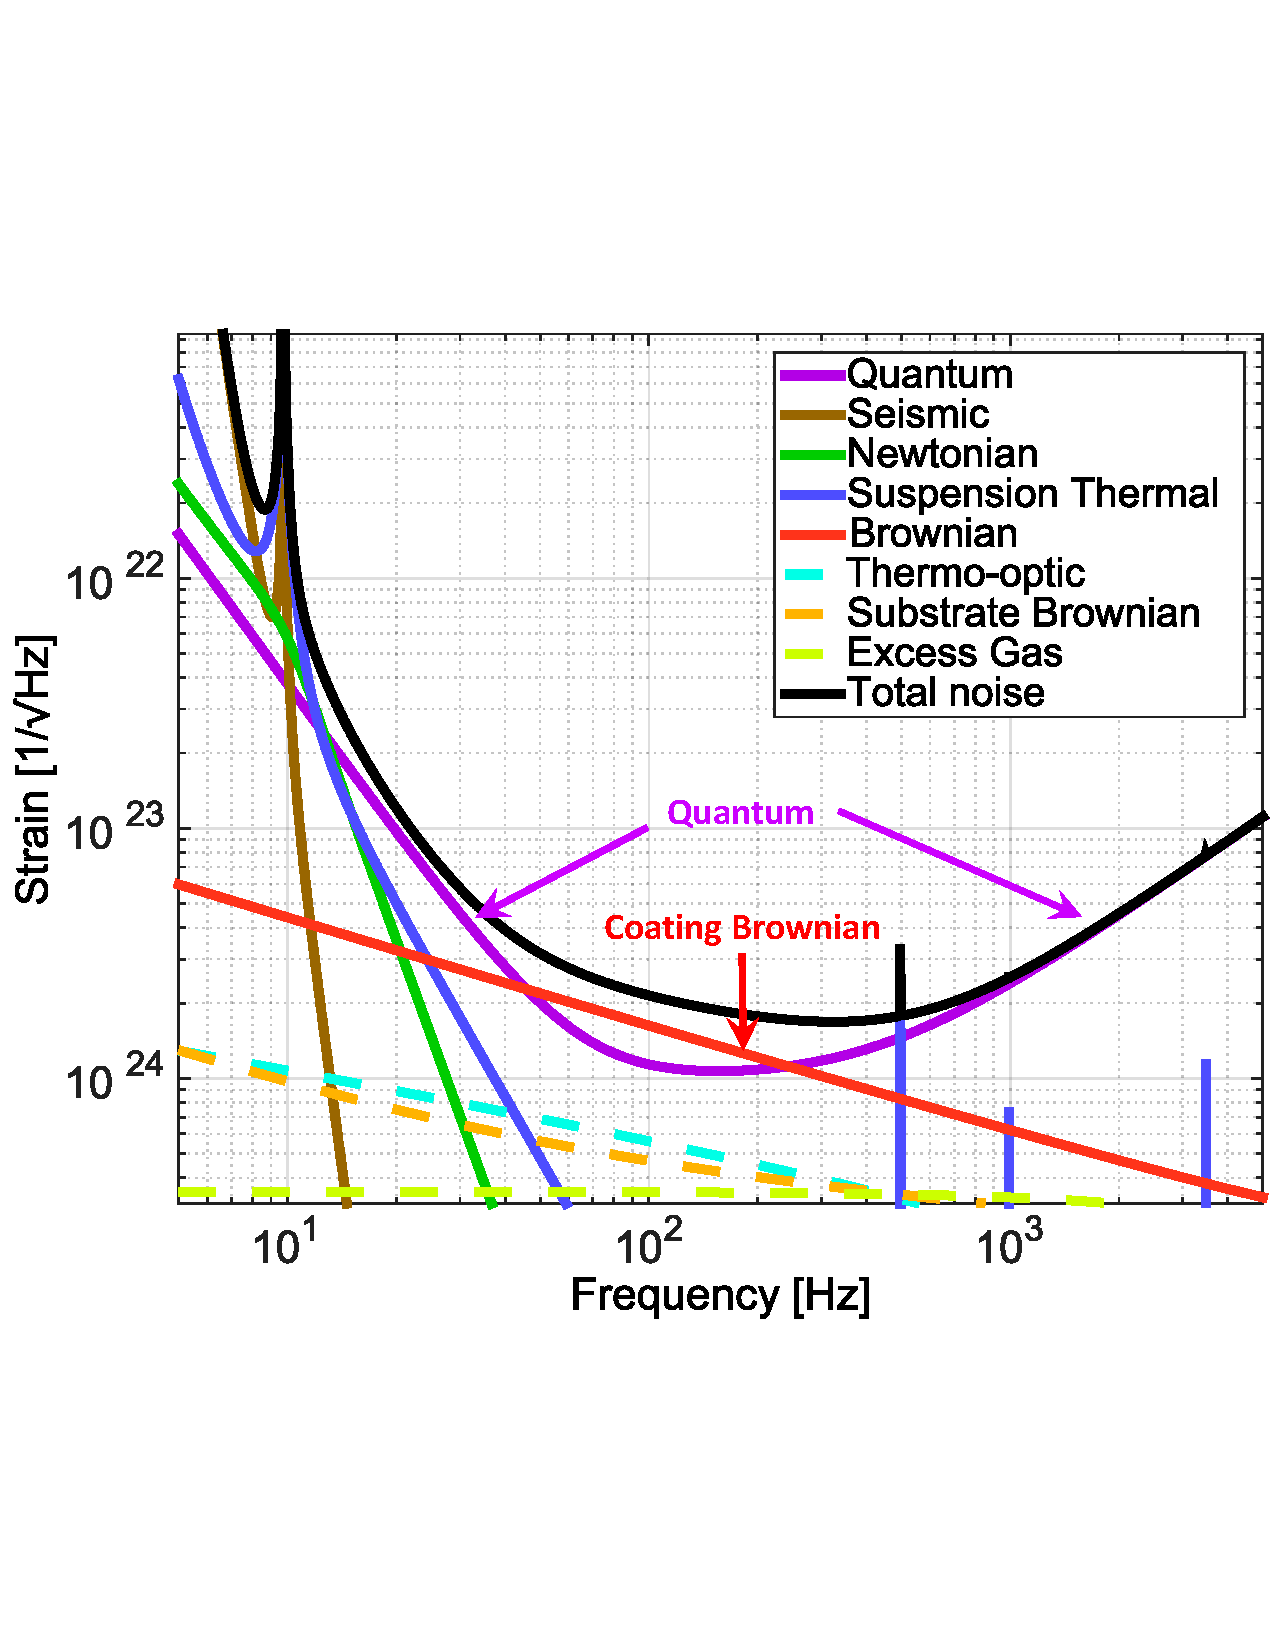
\includegraphics[width=0.7\textwidth]{Figures/APlusBudget.pdf}
%figure from instrument white paper 2020
\caption{Exemplary noise budget for the \acf{a+LIGO} (LIGO Lab/Caltech/MIT)}
\label{A+noisebudget}
\end{figure}

Thermal noise \ref{Box:Thermal},\cite{ThermalNoiseHammond2014} is produced by random displacements of the mirror surfaces in response to thermally fluctuating stresses in the mirror coatings, substrates, and suspensions and it typically dominates at midband frequencies  (ca.~50-200\,Hz). Quantum noise can be roughly divided into \ac{QRPN} and quantum phase noise or \ac{SN} \cite{QuantumNoiseBarsotti2018}. \ac{QRPN}, or quantum back-action noise, arises from the random buffeting of the suspended interferometer mirrors by the quantum mechanical amplitude fluctuations of the light field being used to sense the arm-length. Shot noise results from quantum phase uncertainty: there is a limit to how well the phase difference between two light fields returning from the interferometers arms can be determined. Radiation pressure noise dominates at low frequencies (ca. 10Hz to 50\,Hz) while shot noise dominates at higher frequencies (above ca. 200\,Hz). The standard quantum limit is the noise floor for which the \ac{QRPN} and shot noise are equal at a given power level (typically around 100\,Hz). 
\Ac*{NN} arises from the direct gravitational forces exerted on the interferometer mirrors by nearby changing mass distributions primarily caused by density fluctuations of the surrounding earth due to seismic waves as well as low frequency atmospheric density changes \cite{InfrasoundNewtonianNoise2018}. 
The test masses cannot be shielded against these fluctuating forces.  In addition to the noise sources discussed above, another important issue is the suppression of instabilities that arise from photon pressure at high optical power. 

In reality there are a myriad of technical noise sources that need to suppressed in order to reveal the 'fundamental limitations' (scattered light, electronic noise, various other control noises)  This is dramatically demonstrated in  figure \ref{fig:aLIGO_Noises} which shows the noise anatomy for the \acf{aLIGO} detector at Livingston, \ac{USA},  circa March 2020.  Much  of the effort and focus when commissioning  a detector is devoted to suppressing such "technical"  noise.
\begin{figure}
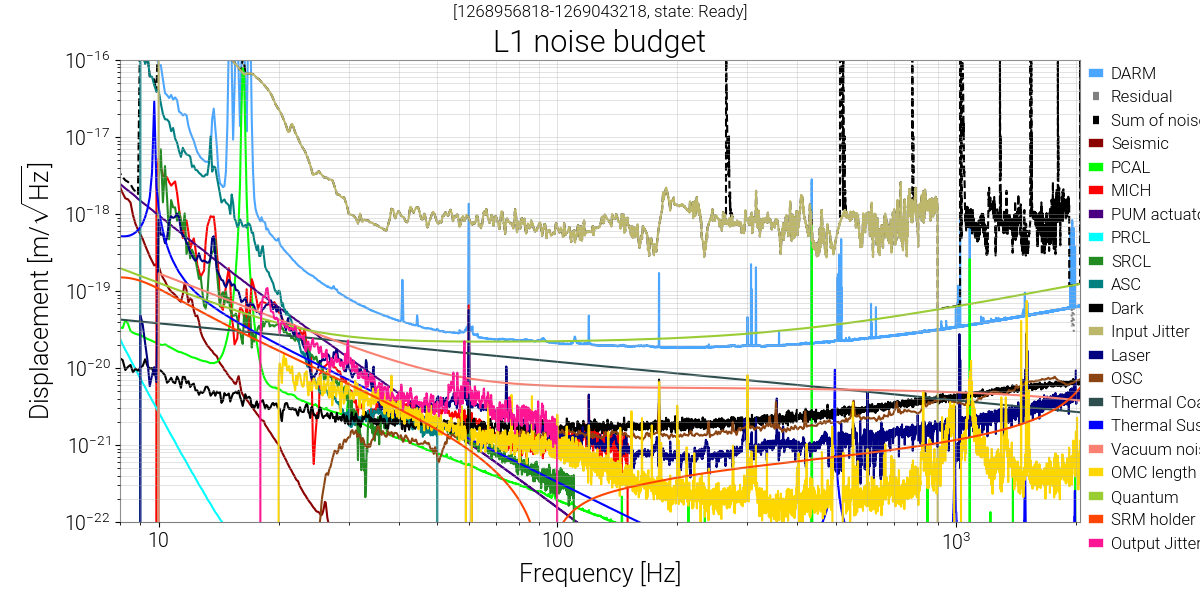
\includegraphics[width=\textwidth]{Figures/L1-READY_7A4FE0_NOISE_BUDGET-1268956818-86400.png}
% dummy picture taken from https://ldas-jobs.ligo-la.caltech.edu/~detchar/summary/day/20200302/isc/noise_budget/#gallery-1 needs to be replaced by a proper noise projection
\caption{Example noise budget for the \acf{aLIGO} interferometer in Livingston, Louisiana, circa March 2020. For details see~\cite{} }
\label{fig:aLIGO_Noises}
\end{figure}
%\vspace{11cm}
%\end{tcolorbox}

From Figure \ref{A+noisebudget}it is clear that the impact on the sensitivity of reducing one noise source depends on other noise contributions at relevant frequencies.  
For example, lowering quantum noise around 100\,Hz will have little impact unless coating Brownian noise is similarly reduced.  The low frequency band below 20\,Hz is far more complex.  
In this report we will review each noise source and the R\&D that needs to be done independently.   
It is beyond the scope of this report to reflect on what may happen if progress on a particular subsystem is slower than expected.  
Such impact on the science that can be done will be considered in trade studies that will be carried out in the various detector collaborations.